\documentclass[aspectratio=169]{beamer}
\usepackage[utf8x]{inputenc}
\usepackage[english]{babel}
\usepackage{hyperref}
\usepackage{minted}
%%\usemintedstyle{perldoc}
\usetheme{default}
\beamertemplatenavigationsymbolsempty{}

\title{U+1F5A8: the Emoji that Killed Chrome!!}
\author{Julian Squires}
\date{May 6th, 2017}
\begin{document}

\begin{frame}
  \titlepage{}
\end{frame}

\begin{frame}
  \begin{center}
    %%\titlepage{}
    %% slack screenshots: chrome crash worldwide
    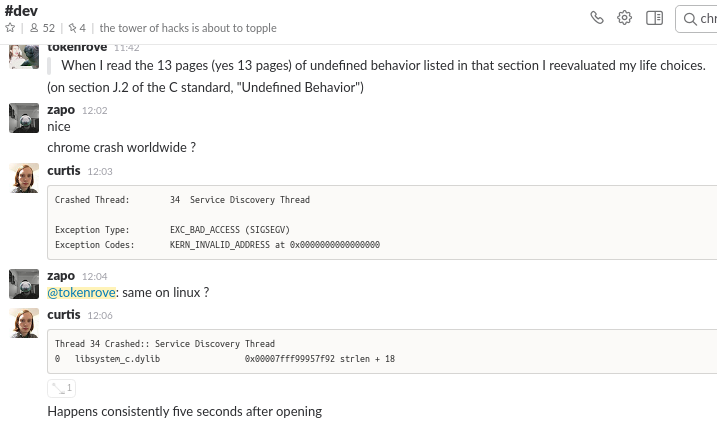
\includegraphics[scale=0.5]{01-chrome-crash-worldwide}
  \end{center}
\end{frame}

\begin{frame}
  \begin{columns}[t]
    \column{0.5\textwidth}\centering
    %% slack screenshots: just plugged in the printer
    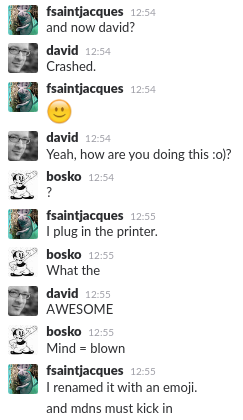
\includegraphics[scale=0.5]{04-plugged-in-the-printer}
    \column{0.5\textwidth}\centering
    %% picture of M402dw
    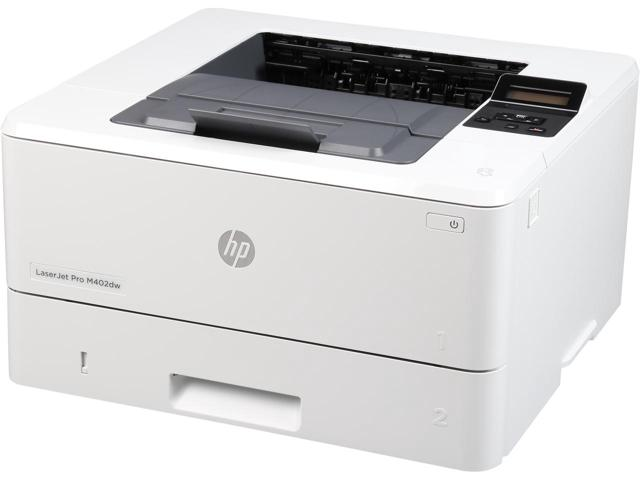
\includegraphics[scale=0.25]{hp-m402dw}
  \end{columns}
\end{frame}

\begin{frame}
  %% this is the greatest day of my life
  \begin{center}
    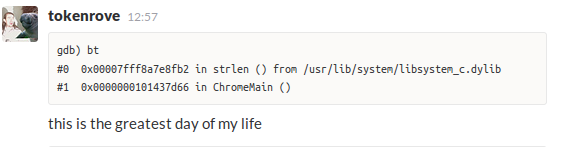
\includegraphics[scale=0.5]{greatest-day}
  \end{center}
\end{frame}

\begin{frame}
  \begin{center}
    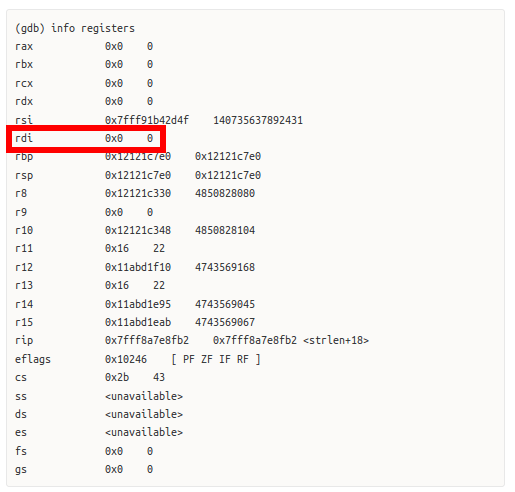
\includegraphics[scale=0.5]{info-registers}
  \end{center}
\end{frame}

\begin{frame}[fragile]
  %% tcpdump
\begin{verbatim}
14:31:38.508375 IP 192.168.5.244.5353 > 224.0.0.251.5353: 0*- [0q] 1/0/0
  PTR M-pM-^_M-^VM-(downstairs._privet._tcp.local. (59)

14:31:39.122765 IP 192.168.5.244.5353 > 224.0.0.251.5353: 0*- [0q] 2/0/4
  (Cache flush) TXT "txtvers=1" "UUID=50484256-4330-3130-3031-5820b14f2d90"
  "ty=M-pM-^MM- M-=M-pM-^MM-6M-( downstairs" "url=https://www.google.com/cloudprint"
  "type=printer" "id=6290b76b-d061-2e84-14eb-dd1f63c06199" "cs=online",
  (Cache flush) SRV NPI4F2D90.local.:80 0 0 (348)
\end{verbatim}
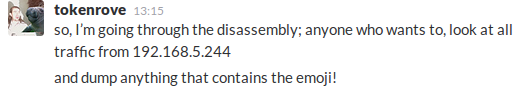
\includegraphics[scale=0.5]{dump-anything-with-the-emoji}
\begin{center}
\end{center}

\end{frame}

\begin{frame}[fragile]
  %% mDNS
  %% printer emoji
  \begin{center}
    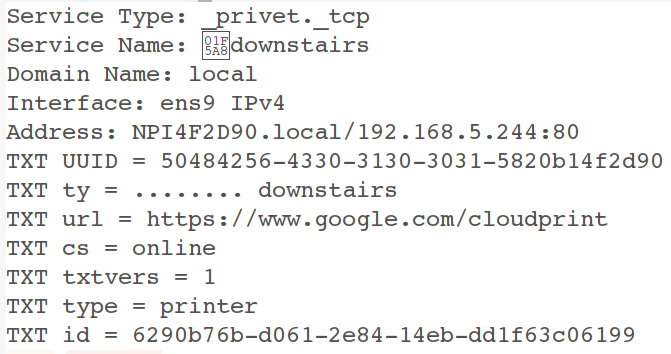
\includegraphics[scale=0.6]{mdns-record}
  \end{center}
\end{frame}

\begin{frame}[fragile]
  %%\frametitle{tcpreplay}
  \begin{minted}[]{shell}
#!/bin/bash

if [ $# -ne 1 ]; then
    echo "Usage:"
    echo "$0 <ethernet interface>"
    exit 1
fi

xxd -r <<EOF | sudo tcpreplay -i $1 -t -
00000000: d4c3 b2a1 0200 0400 0000 0000 0000 0000  ................
00000010: 0000 0400 0100 0000 0a25 be56 d7c1 0700  .........%.V....
00000020: 6500 0000 6500 0000 0100 5e00 00fb 5820  e...e.....^...X
00000030: b14f 2d90 0800 4500 0057 cb83 0000 ff11  .O-...E..W......
00000040: 487a c0a8 05f4 e000 00fb 14e9 14e9 0043  Hz.............C
00000050: 9a8a 0000 8400 0000 0001 0000 0000 075f  ..............._
00000060: 7072 6976 6574 045f 7463 7005 6c6f 6361  privet._tcp.loca
00000070: 6c00 000c 0001 0000 1194 0011 0ef0 9f96  l...............
00000080: a864 6f77 6e73 7461 6972 73c0 0c0b 25be  .downstairs...%.
00000090: 568d df01 0086 0100 0086 0100 0001 005e  V..............^
000000a0: 0000 fb58 20b1 4f2d 9008 0045 0001 78cd  ...X .O-...E..x.
000000b0: cb00 00ff 1145 11c0 a805 f4e0 0000 fb14  .....E..........
000000c0: e914 e901 649e 1900 0084 0000 0000 0200  ....d...........
000000d0: 0000 040e f09f 96a8 646f 776e 7374 6169  ........downstai
000000e0: 7273 075f 7072 6976 6574 045f 7463 7005  rs._privet._tcp.
000000f0: 6c6f 6361 6c00 0010 8001 0000 1194 00b0  local...........
00000100: 0974 7874 7665 7273 3d31 2955 5549 443d  .txtvers=1)UUID=
00000110: 3530 3438 3432 3536 2d34 3333 302d 3331  50484256-4330-31
00000120: 3330 2d33 3033 312d 3538 3230 6231 3466  30-3031-5820b14f
00000130: 3264 3930 1674 793d f08d a0bd f08d b6a8  2d90.ty=........
00000140: 2064 6f77 6e73 7461 6972 7325 7572 6c3d   downstairs%url=
00000150: 6874 7470 733a 2f2f 7777 772e 676f 6f67  https://www.goog
00000160: 6c65 2e63 6f6d 2f63 6c6f 7564 7072 696e  le.com/cloudprin
00000170: 740c 7479 7065 3d70 7269 6e74 6572 2769  t.type=printer'i
00000180: 643d 3632 3930 6237 3662 2d64 3036 312d  d=6290b76b-d061-
00000190: 3265 3834 2d31 3465 622d 6464 3166 3633  2e84-14eb-dd1f63
000001a0: 6330 3631 3939 0963 733d 6f6e 6c69 6e65  c06199.cs=online
000001b0: c00c 0021 8001 0000 0078 0012 0000 0000  ...!.....x......
000001c0: 0050 094e 5049 3446 3244 3930 c028 c0fb  .P.NPI4F2D90.(..
000001d0: 0001 8001 0000 0078 0004 c0a8 05f4 c0fb  .......x........
000001e0: 001c 8001 0000 0078 0010 fe80 0000 0000  .......x........
000001f0: 0000 5a20 b1ff fe4f 2d90 c00c 002f 8001  ..Z ...O-..../..
00000200: 0000 1194 0009 c00c 0005 0000 8000 40c0  ..............@.
00000210: fb00 2f80 0100 0000 7800 08c0 fb00 0440  ../.....x......@
00000220: 0000 08                                  ...
EOF
  \end{minted}
\end{frame}

\begin{frame}[fragile]
  %% UTF-8 assumptions
  %% portion of spec explaining nil return
  \begin{center}
    
\includegraphics[scale=0.5]{what-kind-of-encoding-is-this}
  \end{center}
  \begin{columns}[t]
    \column{0.5\textwidth}\centering
    UTF-8: \verb?F0 9F 96 A8? \\
    \verb?f08d a0bd f08d b6a8? \\
    UTF-8 encoding of \verb?D83D DDA8?
    \vspace*{5em}
    \begin{verbatim}
00000130: 3264 3930 1674 793d f08d a0bd f08d b6a8  2d90.ty=........
00000140: 2064 6f77 6e73 7461 6972 7325 7572 6c3d   downstairs%url=
    \end{verbatim}
    \column{0.3\textwidth}\centering
    \verb?U+1F5A8? \\
    
\includegraphics[scale=0.3]{printer-emoji}
  \end{columns}
\end{frame}

\begin{frame}[fragile]
  \begin{minted}[]{diff}
--- service_discovery_client_mac.mm.old	2016-06-15 07:02:44.590359344 -0400
+++ service_discovery_client_mac.mm	2016-06-15 07:06:22.425805394 -0400
@@ -109,10 +109,11 @@
     if (record_bytes + size <= record_end) {
       VLOG(1) << "TxtRecord: "
               << std::string(record_bytes, static_cast<size_t>(size));
-      output->push_back(
-          [[[NSString alloc] initWithBytes:record_bytes
-                             length:size
-                             encoding:NSUTF8StringEncoding] UTF8String]);
+      NSString* s = [[NSString alloc] initWithBytes:record_bytes
+                                      length:size
+                                      encoding:NSUTF8StringEncoding];
+      if (s != nil)
+        output->push_back([s UTF8String]);
     }
     record_bytes += size;
   }
  \end{minted}
\end{frame}

\begin{frame}
  \begin{center}
    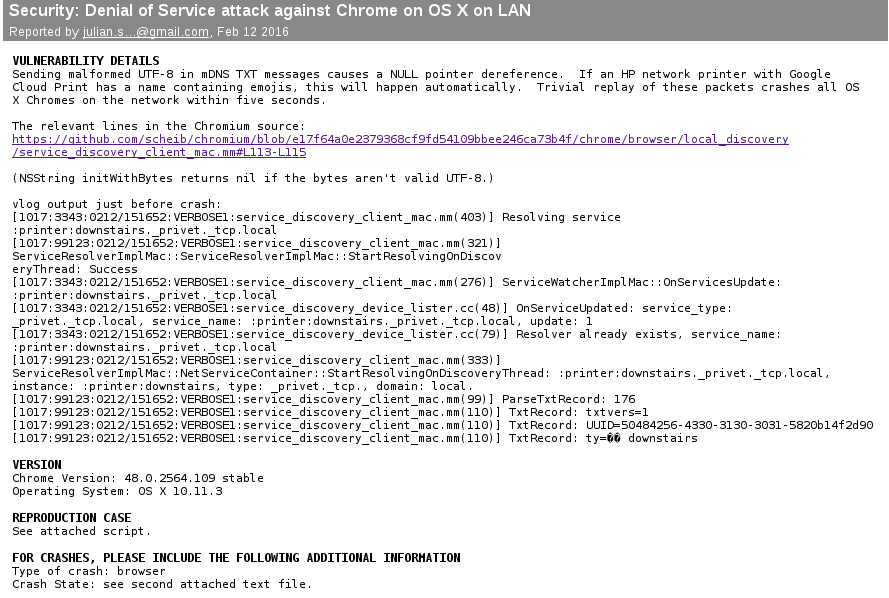
\includegraphics[scale=0.5]{bug-report}
  \end{center}
  %% bug report
\end{frame}

\begin{frame}
  %% bug report
  \begin{center}
    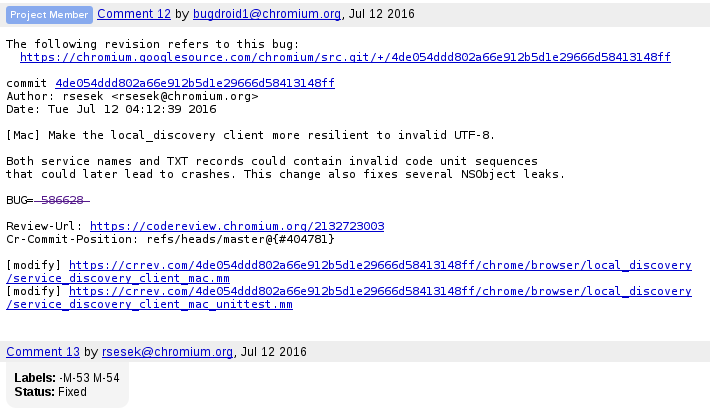
\includegraphics[scale=0.5]{alls-well-that-ends-well}
  \end{center}
\end{frame}

\begin{frame}
  %% why this is exciting
  %% snippets of everything
  %% printer emoji
  \begin{center}
    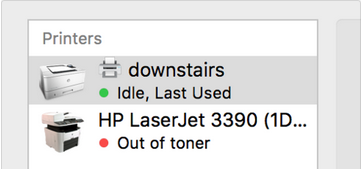
\includegraphics[scale=0.5]{printer-downstairs}
  \end{center}
\end{frame}

\end{document}
